\chapter{Patterns of Enterprise Application Architecture}

Softwareanwendungen, die zu Unternehmenszwecken verwendet werden.

\mparagraph{Eigenschaften}
\begin{compactitem}
    \item Bestenhende Daten. Langlebiger als Anwendung und Hardware
    \item Große Datenmengen.
    \item Gleichzeitiger Zugriff auf die Daten
    \item Schnittstelle zu anderen Systemen
    \item Unterschiedliche Nutzer (erfahren, unerfahren)
    \item Geschäftsregeln und Prozesse sind komplex, aber nicht unbedingt logisch.
\end{compactitem}

\section{Schichten von EA}
\begin{compactitem}
    \item \textbf{Präsentation}: Interaktion von User und Software handhaben. Informationen darstellen und
    Eingaben interpretieren.
    \item \textbf{Domäne}: Datenverarbeitung
    \item \textbf{Data Source}: Kommunikation mit anderen Systemen. Datenbanken etc.
\end{compactitem}

\section{EA Patterns}

\subsection{Domain Logic Patterns}
Wie am besten Geschäftsregeln repräsentieren?
Umsetzung von Geschäftslogik
\subsubsection{Transaction Script}
Organisiere Geschäftslogik in einzelne Prozeduren. Jede Prozedur bearbeitet eine einzelne
Anfrage der Presentationsschicht.
Pro Aufgabe implementiere eine Methode.

+ Einfach \\
+ einfach zu verbinden mit anderen Datenquellen \\
+ Transaktionsgrenzen leicht zu bestimmen. \\
- Skaliert nicht gut mit komplexerer Domänenlogik \\
- Code muss evtl. dupliziert werden

\subsubsection{Domain Model}
Strukturiere Domänenlogik anhand eines Objektmodells sodass Objekte sowohl Verhalten als auch Daten
enthalten. Objekte arbeiten zusammen um Transaktion durchzuführen.

+ Besser bei komplexeren Logik \\
- Verbindung mit Datenquelle komplexer
- Flachere Lernkurve wenn nicht vertraut mit OO ist.

\subsubsection{Table Module}
Einzelne Instanz einer Klasse behandelt die Geschäftslogik für alle Reihen/Zeilen
einer Tabelle oder Views. Pro Tabelle eine Klasse.

+ direktes Mapping auf Daten \\
+ Separiert Logik für verschiedene Konzepte \\
- Keine Objekt Instanzen: kann schlecht für komplexere Logik sein.

\begin{figure}[!h]
    \centering
    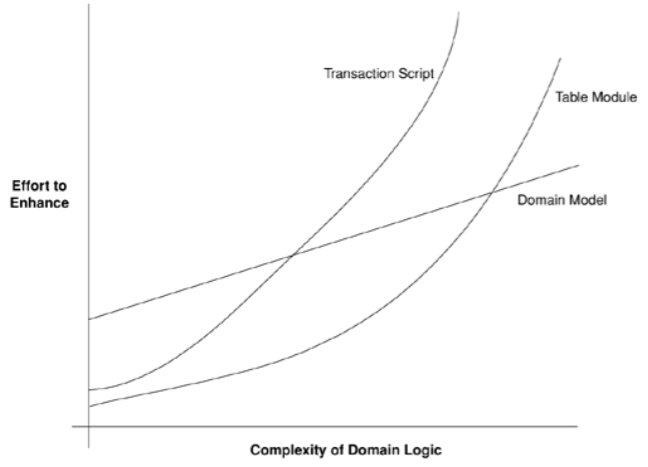
\includegraphics[scale=0.5]{domainlogik}
\end{figure}

\subsection{Data Source Architecture}
Wie Domänen Logik und Datenquelle separieren?
\subsubsection{Record Set}
In-Memory Repräsentation der Daten. Direktes Ergebnis einer SQL-Query

\subsubsection{Table Data Gateway}
Ein Objekt, dass als Gateway zu einer Datenbanktabelle fungiert. Eine Instanz des Table Data Gateway
behandelt alle Reihen der Tabelle. Instaz behinahltet notwendiges SQL für Interaktion mit
kompletter Tabelle.
Trennung von SQL Statements und Code der zugriff auf Daten hat.

Unterschied Facade und Gateway: Spezielle Nutzen vs. allgemeiner Nutzen (facade)

\subsubsection{Active Record}
Ein Objekt, dass eine Reihe aus einer Datenbanktabelle oder View wrapped.
Kapselt Datenbank Zugriff und kann Domänenlogik auf den Daten ausfühen.
Bringt Daten und Funktionalität zusammen.

+ Gut bei sehr einfacher Domänenlogik
- Datenbankschema und Active Record müssen Isomorph sein (1:1 mapping). Schwierigkeiten für
komplexere Logik mit Vererbung

\subsubsection{Row Data Gateway}
Ein Objekt, dient als Gateway eines einzelnen Datensatzes/Zeile einer Datenbank. Eine Instanz pro
Zeile.

Trennung von Datenbank Zugriff und Objekte im Speicher.

\subsubsection{Data Mapper}
Mapper, der Objekte im Speicher auf Datenbank abbilden kann. Beides bleibt komplett unabhängig.
Trennt Datenbank-Logik und Domänenlogik

\subsection{when to use what?}
\begin{compactitem}
    \item \textbf{Transaction Script}:
    \begin{compactitem}
        \item Row Data Gateway: Explizite Schnittstelle, besser weiter zu entwickeln
        \item Table Date Gateway: Wenn Record Set Framework
    \end{compactitem}
    \item \textbf{Domain Model}
    \begin{compactitem}
        \item Simpel: Active Record
        \item Komplexes Mapping: Data Mapper
    \end{compactitem}
    \item \textbf{Table Module} (Wenn Record Set Framework)
    \begin{compactitem}
        \item Table Data Gateway
    \end{compactitem}
\end{compactitem}
\subsection{Object-relational structural pattern}
Wie Objekte auf relationale Datenbank abbilden?
Alle Patterns sind für Domänenmodells mit Data Mapper gedacht.
\subsubsection{Single Table Inheritance}
Repräsentiert Vererbungshierarcie der Klassen als eine einzelne Tabelle welche Spalten mit allen
Feldern der verschiedenen Klassen hat.

+ Komplette Hierarchie in einer Tabelle\\
+ Keine Joins nötig \\
- Verschwendeter Platz für Spalten\\
- Zugriff ist Bottleneck

\subsubsection{Class Table Inheritance}
Eine Tabelle pro Klasse. Attribute sind verteilt

+ Klare Struktur \\
- Schlechte performance
- Benötigt Joins
\subsubsection{Concrete Table Inheritance}
Eine Tabelle pro konkrete Klasse mit allen Attributen.
+ keine Joins nötigt \\
- Finden erfordert mehrere Queries \\
- Änderungen der Superklasse beeinflusst alle anderen Tabellen.
